\documentclass[12pt, a4paper]{report}

% Essential packages
\usepackage{tocloft}
\usepackage{mathptmx}
\usepackage{geometry}
\usepackage{fontspec}
\usepackage{polyglossia}
\usepackage{algorithm}
\usepackage{algpseudocode}
\usepackage{geometry}
\usepackage{graphicx}
\usepackage{amsmath}
\usepackage{amsfonts}
\usepackage{amssymb}
\usepackage{enumerate}
\usepackage{float}
\usepackage{indentfirst}
\usepackage{parskip}
\usepackage{setspace}
\usepackage{minted}
\usepackage{xcolor}
\usepackage{hyperref}
\usepackage{mdframed}
\usepackage{pdfpages}
\usepackage{subcaption}
\usepackage[style=ieee, backend=biber]{biblatex}

% Hyperref
\hypersetup{
    colorlinks=false,
    pdfborder={0 0 0}
}

\usepackage{chngcntr}
\counterwithin{figure}{section}
\counterwithin{table}{section}

\usepackage[math-style=TeX]{unicode-math}

\raggedbottom

% Language setup
\setmainlanguage{english}
\setotherlanguage{khmer}
\setmainfont{Times New Roman}
\setmathfont{STIX Two Math}
\newfontfamily\khmerfont{Khmer OS Siemreap}[Script=Khmer]
\newfontfamily\khmermoul{Khmer OS Muol Light}[Script=Khmer]

% Page setup
\geometry{margin=1in}

% Formatting the Table of Contents
\renewcommand{\cftsecfont}{}
\renewcommand{\cftsubsecfont}{}
\renewcommand{\cftsubsubsecfont}{}
\renewcommand{\cftsecpagefont}{}
\renewcommand{\cftsubsecpagefont}{}
\renewcommand{\cftsubsubsecpagefont}{}
\renewcommand{\cftsecleader}{\cftdotfill{\cftdotsep}} % Ensure dots for sections
\renewcommand{\cftsubsecleader}{\cftdotfill{\cftdotsep}}
\renewcommand{\cftsubsubsecleader}{\cftdotfill{\cftdotsep}}

% section title space
\setlength{\cftsecnumwidth}{2em}
\setlength{\cftsubsecnumwidth}{2.5em}
\setlength{\cftsubsubsecnumwidth}{3em}

% Set the numbering depth
\setcounter{secnumdepth}{3}
\setcounter{tocdepth}{3}


% Other settings
\setlength{\parskip}{0pt}
\setlength{\parindent}{1.5em}
% Set spacing vertical line
\setstretch{1.5}
% Title formatting for sections, subsections, and subsubsections
\usepackage{titlesec}

% Section formatting
\titleformat{\section}[block]
  {\normalfont\fontsize{14}{16}\selectfont\bfseries}
  {\thesection}
  {1em}
  {}

% Subsection formatting
\titleformat{\subsection}
  {\normalfont\fontsize{12}{14}\selectfont\bfseries}
  {\thesubsection}
  {1em}
  {}

% Subsubsection formatting
\titleformat{\subsubsection}
  {\normalfont\fontsize{12}{14}\selectfont\bfseries}
  {\thesubsubsection}
  {1em}
  {}

\newcommand{\specialsection}[1]{%
  \section*{\centering\fontsize{14}{16}\selectfont\bfseries\uppercase{#1}}%
  \addcontentsline{toc}{section}{#1}%
}

\addbibresource{references/references.bib}
\DefineBibliographyStrings{english}{bibliography = {References}}

% Custom format for List of Figures
\renewcommand{\cftfigpresnum}{Figure }
\renewcommand{\cftfigaftersnum}{ }
\setlength{\cftfignumwidth}{5em}  % Increased width for figure numbers
\renewcommand{\cftfigdotsep}{\cftdotsep}
\setlength{\cftbeforefigskip}{0.5em}

% Custom format for List of Tables
\renewcommand{\cfttabpresnum}{Table }
\renewcommand{\cfttabaftersnum}{ }
\setlength{\cfttabnumwidth}{5em}  % Increased width for table numbers
\renewcommand{\cfttabdotsep}{\cftdotsep}
\setlength{\cftbeforetabskip}{0.5em}

% Ensure figures and tables are numbered within sections
\counterwithin{figure}{section}
\counterwithin{table}{section}

% Redefine figure and table numbering format
\renewcommand{\thefigure}{\thesection.\arabic{figure}}
\renewcommand{\thetable}{\thesection.\arabic{table}}

% Remove "Figure" or "Table" from actual captions
\captionsetup[figure]{labelformat=simple, labelsep=space}
\captionsetup[table]{labelformat=simple, labelsep=space}

% Adjust spacing and formatting of List of Figures and Tables
\setlength{\cftfigindent}{0pt}
\setlength{\cfttabindent}{0pt}
\renewcommand{\cftfigfont}{\normalfont}
\renewcommand{\cfttabfont}{\normalfont}

% Define GitHub-like colors
\definecolor{gh-bg}{HTML}{ffffff}
\definecolor{gh-text}{HTML}{24292e}
\definecolor{gh-keyword}{HTML}{d73a49}
\definecolor{gh-string}{HTML}{032f62}
\definecolor{gh-comment}{HTML}{6a737d}

% Set up minted style for Python
\setminted[python]{
  style=default,
  bgcolor=gh-bg,
  fontsize=\small,
  frame=single,
  framesep=2mm,
  rulecolor=\color{gh-text!20},
  breaklines=true,
  breakanywhere=true,
  tabsize=4,
  autogobble=true,
  baselinestretch=1.2,
  fontfamily=ttfamily,
  linenos=false,
}

% Custom command for Python code
\newenvironment{pythoncode}
 {\VerbatimEnvironment
  \begin{minted}[
    bgcolor=gh-bg,
    fontsize=\footnotesize,
    breaklines=true,
    breakanywhere=true,
    fontfamily=ttfamily,
    frame=single,
    framesep=2mm,
    rulecolor=\color{gh-text!20},
    baselinestretch=1.2,
    linenos=false,
  ]{python}}
 {\end{minted}}

% Command for centered special sections
\newcommand{\centeredsection}[1]{%
  \clearpage
  \phantomsection
  \addcontentsline{toc}{section}{#1}
  \begin{center}
    \fontsize{14}{16}\selectfont\bfseries\uppercase{#1}
  \end{center}
  \vspace{1em}
}

% Command for non-centered special sections
\newcommand{\regularsection}[1]{%
  \clearpage
  \phantomsection
  \addcontentsline{toc}{section}{#1}
  {\fontsize{14}{16}\selectfont\bfseries\uppercase{#1}}
  \vspace{1em}
}

% Customize specific elements
\AtBeginEnvironment{minted}{
  \renewcommand{\fcolorbox}[4][]{\colorbox{#4}{#3}}
}

\defbibheading{bibliography}[\refname]{%
  \clearpage
  \phantomsection
  \addcontentsline{toc}{section}{\refname}
  \begin{center}
    \fontsize{14}{16}\selectfont\bfseries\uppercase{\refname}
  \end{center}
  \vspace{20pt}
}

\begin{document}
% Title Page
% Replace Cover.pdf with your own cover/title pages (same page count, or adjust the range below).

\includepdf[pages={1,2,3}]{Cover.pdf}

\pagenumbering{roman}

%% Acknowledgement
\centeredsection{ACKNOWLEDGEMENT}
\noindent\hspace*{\parindent} Thank the people who supported your thesis work: family, your institution's leadership, your department head, your advisor, and anyone else who helped. One paragraph per person or group works well, as shown in this example structure.

Thank your family or sponsors for their support.

Thank your institution's director/leadership, e.g. \textbf{Dr. FIRSTNAME LASTNAME}, Director of \textit{Your Institution}.

Thank your department head and faculty, e.g. \textbf{Dr. FIRSTNAME LASTNAME}, Head of \textit{Your Department}.

Thank your thesis advisor, e.g. \textbf{Mr./Ms./Dr. FIRSTNAME LASTNAME}.

Thank friends, peers, or anyone else who helped along the way.
\clearpage

%% Summary in Khmer
\section*{\centerline{\texorpdfstring{%
    \begin{khmer}%
    \khmermoul\fontsize{14}{16}\selectfont សេចក្តីសង្ខេប%
    \end{khmer}%
}{សេចក្តីសង្ខេប}}}
\addcontentsline{toc}{section}{\texorpdfstring{\khmermoul សេចក្តីសង្ខេប}{សេចក្តីសង្ខេប}}
% Khmer text using the defined Khmer fonts (\khmerfont, \khmermoul)
\begin{khmer}
\noindent\hspace*{\parindent}សូមសរសេរសេចក្តីសង្ខេបនៃការស្រាវជ្រាវរបស់អ្នកជាភាសាខ្មែរនៅទីនេះ។ អក្សរខ្មែរដែលសរសេរនៅក្នុងបរិយាកាស khmer នេះនឹងបង្ហាញបានត្រឹមត្រូវ។
\end{khmer}
\clearpage

%% Resume (French summary -- optional, remove if not required)
\centeredsection{RESUME}
\noindent\hspace*{\parindent} Write your thesis summary in French here. This section is optional; remove it if your institution does not require a French summary.
\clearpage

%% Abstract
\centeredsection{ABSTRACT}
\noindent\hspace*{\parindent}Write your thesis abstract in English here: the research problem, your approach, and your key results and conclusions. One or two short paragraphs is typical.
\clearpage

% Abbreviations and symbols
\centeredsection{ABBREVIATIONS AND SYMBOLS}
\begin{tabbing}
  \hspace{2cm} \= \kill
  \textbf{Abbreviations:} \\
  ABC \> Example abbreviation \\
  XYZ \> Another example abbreviation \\
  \\
  \textbf{Symbols:} \\
  $x$ \> Example variable \\
  $\alpha$ \> Example parameter \\
\end{tabbing}

% Add List of Figures and List of Tables to TOC
\addcontentsline{toc}{section}{List of Figures}
\addcontentsline{toc}{section}{List of Tables}

% Table of Contents
\renewcommand{\cfttoctitlefont}{\hfil\fontsize{14}{16}\selectfont\bfseries}
\setlength{\cftbeforetoctitleskip}{-50pt}
\setlength{\cftaftertoctitleskip}{20pt}
\renewcommand{\contentsname}{TABLE OF CONTENTS}

% List of Figures
\renewcommand{\cftloftitlefont}{\hfil\fontsize{14}{16}\selectfont\bfseries}
\setlength{\cftbeforeloftitleskip}{-50pt}
\setlength{\cftafterloftitleskip}{20pt}
\renewcommand{\listfigurename}{LIST OF FIGURES}

% List of Tables
\renewcommand{\cftlottitlefont}{\hfil\fontsize{14}{16}\selectfont\bfseries}
\setlength{\cftbeforelottitleskip}{-50pt}
\setlength{\cftafterlottitleskip}{20pt}
\renewcommand{\listtablename}{LIST OF TABLES}

% Table of Contents
\tableofcontents
\clearpage

% List of Figures
\listoffigures
\clearpage

% List of Tables
\listoftables
\clearpage

% Reset section numbering to 0
\setcounter{section}{0}
\renewcommand\thesection{\arabic{section}}
\renewcommand\thesubsection{\thesection.\arabic{subsection}}
\renewcommand\thesubsubsection{\thesubsection.\arabic{subsubsection}}

%% Body
\pagenumbering{arabic}

\section{Introduction}

\noindent\hspace*{\parindent} Start your introduction here. Explain the background of your problem, why it matters, and what gap in existing work your thesis addresses.

\subsection{Background}
\noindent\hspace*{\parindent} Describe the context and prior work related to your topic. Cite sources using \texttt{\textbackslash cite\{\}}, for example \cite{williams2017information}.

\subsection{Problem Statement}
\noindent\hspace*{\parindent} State clearly what problem your thesis solves.

\subsection{Objectives}
\noindent\hspace*{\parindent} List the objectives of your research, e.g. using an itemized list:
\begin{itemize}
    \item First objective.
    \item Second objective.
    \item Third objective.
\end{itemize}

\subsection{Thesis Structure}
\noindent\hspace*{\parindent} Briefly outline how the rest of the thesis is organized (one sentence per chapter/section is typical).

\begin{figure}[H]
    \centering
    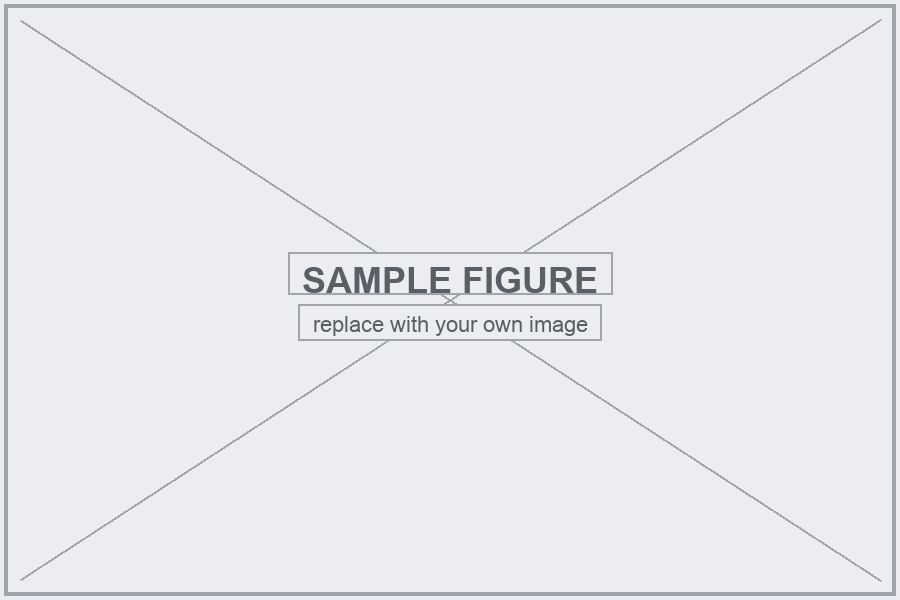
\includegraphics[width=0.6\textwidth]{figure/sample-figure.png}
    \caption{Example figure -- replace with a diagram of your own, e.g. an overview of your thesis concept}
    \label{fig:intro-overview}
\end{figure}


\section{Methodology}

\subsection{Overview}
\noindent\hspace*{\parindent} Describe your overall approach or system design here.

\subsection{Example: Equation}
\noindent\hspace*{\parindent} Mathematical formulations use standard \texttt{amsmath} / \texttt{unicode-math} syntax, for example a state-space model:

\begin{equation}
    \dot{x}(t) = f\big(x(t), u(t)\big)
    \label{eq:example-dynamics}
\end{equation}

\noindent\hspace*{\parindent} where $x$ is the state vector and $u$ is the control input vector.

\subsection{Example: Figure}
\noindent\hspace*{\parindent} Figures are numbered per section (e.g. Figure~1.1 in Section~1) and listed in the List of Figures automatically.

\begin{figure}[H]
    \centering
    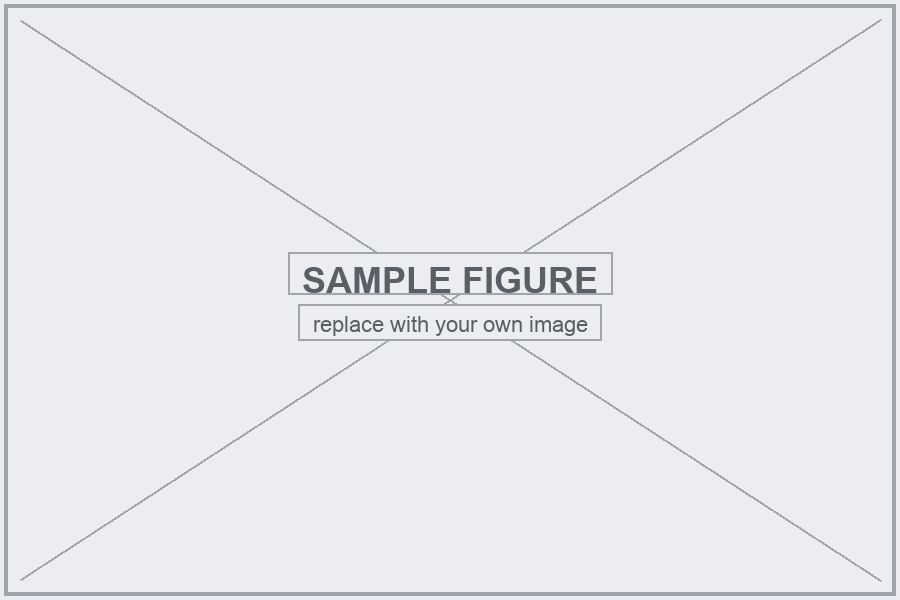
\includegraphics[width=0.6\textwidth]{figure/sample-figure.png}
    \caption{Example figure -- replace with your own diagram or plot}
    \label{fig:methodology-example}
\end{figure}

\subsection{Example: Table}
\noindent\hspace*{\parindent} Tables follow the same numbering convention as figures.

\begin{table}[H]
    \centering
    \caption{Example parameter table}
    \begin{tabular}{|l|c|}
    \hline
    \textbf{Parameter} & \textbf{Value} \\
    \hline
    Example parameter A & $1.0$ \\
    \hline
    Example parameter B & $0.5$ \\
    \hline
    \end{tabular}
    \label{table:example-params}
\end{table}

\subsection{Example: Algorithm}
\noindent\hspace*{\parindent} Pseudocode uses the \texttt{algorithm}/\texttt{algpseudocode} packages.

\begin{algorithm}[H]
    \caption{Example Algorithm}
    \begin{algorithmic}[1]
        \State Initialize variables
        \For{$i \gets 1$ \textbf{to} $N$}
            \State Perform an update step
        \EndFor
        \State \textbf{return} result
    \end{algorithmic}
\end{algorithm}

\subsection{Example: Code Block}
\noindent\hspace*{\parindent} Python code blocks use the custom \texttt{pythoncode} environment (syntax highlighting via \texttt{minted}).

\begin{pythoncode}
def example_function(x, u):
    """Replace with your own code example."""
    return x + u
\end{pythoncode}


\section{Results and Discussion}

\subsection{Experimental Setup}
\noindent\hspace*{\parindent} Describe your experimental setup, dataset, or simulation environment here.

\subsection{Results}
\noindent\hspace*{\parindent} Present your results here, referring to figures and tables as needed, e.g. see Figure~\ref{fig:results-example} and Table~\ref{table:results-example}.

\begin{figure}[H]
    \centering
    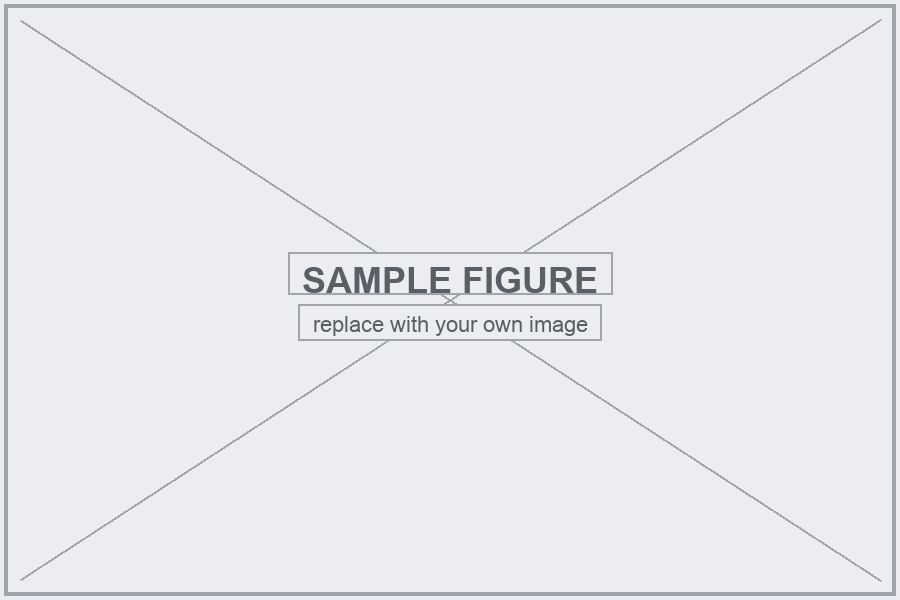
\includegraphics[width=0.6\textwidth]{figure/sample-figure.png}
    \caption{Example results figure -- replace with your own plot}
    \label{fig:results-example}
\end{figure}

\begin{table}[H]
    \centering
    \caption{Example results comparison}
    \begin{tabular}{|c|c|c|}
    \hline
    \textbf{Method} & \textbf{Metric A} & \textbf{Metric B} \\
    \hline
    Baseline & $0.00$ & $0.00$ \\
    \hline
    Proposed & $0.00$ & $0.00$ \\
    \hline
    \end{tabular}
    \label{table:results-example}
\end{table}

\subsection{Discussion}
\noindent\hspace*{\parindent} Interpret your results here: what do they mean, how do they compare to prior work (cite as needed, e.g. \cite{Salzmann_2023}), and what are the limitations?


\section{Conclusion and Future Work}

\noindent\hspace*{\parindent} Summarize your thesis here: what you did, what you found, and how it addresses the objectives stated in the introduction.

\noindent\hspace*{\parindent} Discuss the limitations of your work and suggest directions for future research.


\printbibliography[heading=bibliography]

\end{document}
